\documentclass[twocolumn,letterpaper]{article}
%% If you use dvips and ps2pdf, please use Postscript font
%% and uncomment the line below.
\usepackage{times}
\usepackage{graphicx}
\usepackage{epstopdf}
\usepackage{amssymb}
\usepackage{amsmath}
\usepackage{amsthm}
\usepackage{longtable}
\usepackage{tabularx}
\usepackage{graphicx}
\usepackage{array}
\usepackage{tabu}
\usepackage{CJK}
\usepackage{float}
\usepackage{subcaption}
\usepackage{eqnarray}
%%%%%%%%%%%%%%%%%%%%%%%%%%%%%%%%%%%%%%%%%%%%%%%%%%%%%%%%%%%%%%%%%%%%%%%
\usepackage{aspdac2e}
\usepackage{pbox}

\begin{document}
%date not printed
\date{}

%make title
\title{\Large\textbf{Efficient Photovoltaic Module Models} }	

%for single author
%\author{Center the Authors Names Here \\
%Center the Affiliations Here\\
%Center the City, States and Country Here\\
%{\small (it is your option if you want your entire address listed)}}

%for two authors
\author{\normalsize
 \begin{tabular}[t]{c@{\extracolsep{8em}}c}
  \large Author Name& \large Coauthor Name \\
  \\
   Author Department & Coauthor Department \\
   Author Institute  & Coauthor Institute \\
   City, ST~~zipcode & City, ST~~zipcode\\
   Tel: 123-456-7890 & Tel: +81-3-333-1234\\
   Fax: 123-456-0987 & Fax: +81-3-333-5678\\
   e-mail: aaa@bbb.ccc.ddd & e-mail eee@ffff.ggg.hh\\
\end{tabular}}

\maketitle

\thispagestyle{empty}

\begin{abstract}

\small\bf Abstract---
Bypass diodes are added to photovoltaic (PV) modules to compensate for power loss under shading effects. However, existing models cannot efficiently model PV modules with bypass diodes. In this paper, we develop an efficient Colony-Wise model with the nearly the same accuracy as the Ground Truth (GT) model, but its calculating time is reduced by $5.81$ times on average. Furthermore, a more efficient N-Colony model is proposed, which has an average $5.15\%$ maximum power point error, and an average power-voltage curve correlation of $0.96$, and uses about $1/16$ calculating time when compared to the GT model. To the best of our knowledge, the Colony-Wise model and the N-Colony model are the two most efficient models for real-time solar energy prediction.
\end{abstract}



\section{Introduction}
As a promising solution in the clean energy, photovoltaic (PV) systems have drawn great attention recently. An accurate PV system model is the kernel in the PV system optimization. Furthermore, a fast and accurate model is more attractive when real time applications, such as to capture the PV system characteristics with ever-changing shadings \cite{koutroulis2001development, xiao2004modified}, are required.

A PV system model needs to consider mismatches across solar cells in PV systems. Mismatches have to be considered for two reasons. First, a PV system has numerous solar cells - a PV system consists of thousands of PV modules, and each PV module consists of cascaded and paralleled solar cells. Thus, solar cell mismatches are inevitable. Second, PV systems are vulnerable to mismatches. Mismatches, such as temperature variations, non-uniform cell aging, and non-uniform shading across the cells, can cause power losses and solar cell damages \cite{herrmann1997hot}. The non-uniform shading is also known as the Shading Effects \cite{shading1, sullivan1965shadow}. Shading Effects lead to the largest output power reduction and cell damage \cite{shading1}. Furthermore, the shading on PV module is always changing. It needs a fast PV system model.

The bypass diode is another essential part in a PV module, and has to be modeled accurate in a PV module model. Bypass diodes are connected in parallel to solar cells. Figure \ref{fig:colexample} shows a solar cell chain with $3$ bypass diodes. Bypass diodes have been proven to be an effective solution to compensate for consequences cause by mismatches \cite{bp1}.

%insert figure 1
\begin{figure}[tb]
    \centering
    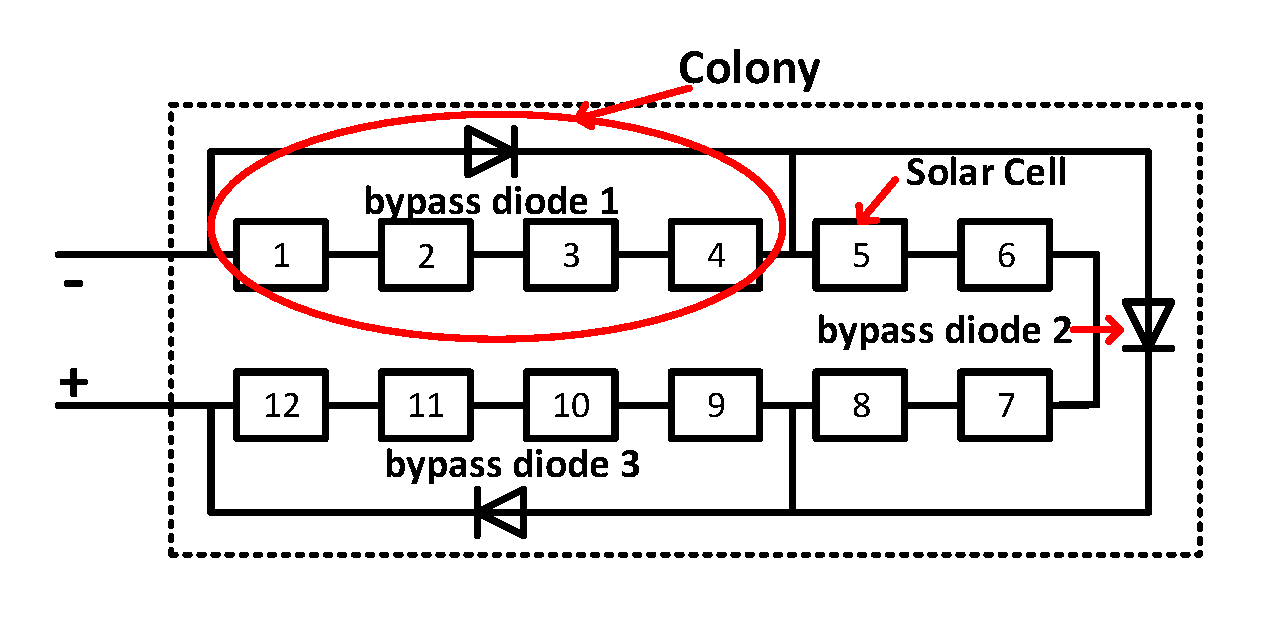
\includegraphics[width=1\columnwidth]{figs/colony_example_new.pdf}
    \caption{A PV module with 1 solar cell chain, which consists of 12 solar cells and 3 colonies.}
    \label{fig:colexample}
\end{figure}

A PV system��s model is based on PV module models. The existing PV module models are equivalent circuit models \cite{oneD1, oneD3}. Generally, a solar cell is modeled as a circuit, with a current source, diodes and resistors. A well-accepted solar cell model is shown in Figure \ref{fig:oneD}. It is referred to as the \textit{One-Diode model} in this paper. A PV module model is then modeled by cascaded and paralleled One-Diode solar cell models, along with the bypass diodes according to the PV module��s configuration. Each One-Diode solar cell has its own parameters to model mismatches. This PV module model offers great accuracy. We refer this model as the \textit{Ground Truth (GT)} model throughout this paper. An example is as in Figure \ref{fig:colexample}. It is a PV module with a single solar cell chain that consists of $12$ solar cells and $3$ bypass diodes. Therefore, its GT model has $12$ One-Diode models and $3$ diode models. The major drawback of the GT model is its computational time. The GT model��s complexity is proportional to the number of solar cells. Consequently, the reduction of PV module model��s complexity is appealing.

\begin{figure}[tb]
    \centering
    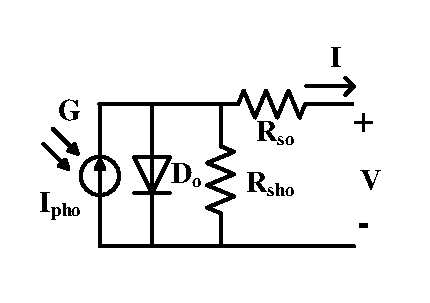
\includegraphics[width=0.7\columnwidth]{figs/one_diode_diagram.pdf}
    \caption{The One-Diode model of a solar cell.}
    \label{fig:oneD}
\end{figure}

In this paper, we propose two PV module models to solve the above problem. The first model is call the \textit{Colony-Wise (CW)} model. A \textit{colony} is defined as a bypass diode plus all its paralleled solar cells, as shown in the circle in Figure \ref{fig:colexample}. The number of colonies inside a PV module equals its quantity of bypass diodes. Solar cells inside of each colony are lumped into at most two \textit{macro cells}. The macro cell is modeled as the One-Diode model. Compared with the GT model, the CW model remains high accuracy, while its complexity is only proportional to the number of bypass diodes in a PV module.

We proposed a second \textit{N-Colony (NC)} model to further reduce the complexity. The N-Colony model models a PV module with at most N colonies, where N is the number of bypass diodes in a module��s cascaded solar cell chain. All solar cells inside each colony are only modeled by one \textit{super cell}. This super cell is again modeled by the One-Diode model. The NC model achieves constant computational complexity with acceptable accuracy.

Our major contribution is that these two models can model PV module of various configurations and with shading effects accurately and efficiently.

The rest of this paper is organized as follows. Section II presents the One-Diode solar cell model, and how to represent shading effects and PV module configurations. These are the preliminaries of our proposed PV module models. Section III and Section IV introduce and validate the Colony-Wise model and the N-Colony Model respectively. Section V compares these two new models with the Ground Truth model. Finally, Section VI concludes the paper.


\section{Preliminaries}
\subsection{The One-Diode Solar Cell Model}
A well-accepted way to model a solar cell is through an equivalent circuit \cite{oneD1}. This model is also denoted as the One-Diode model in the paper. It has one current source and a diode in parallel as shown in Figure \ref{fig:oneD} in Section I.

For the One-Diode model, the Current-Voltage (I-V) curve of the solar cell is as the following:
\begin{equation}\label{equ:oneD}
  I = I_{ph_o} - I_{s_o}[exp(q\frac{V + R_{s_o}I}{N_okT}) - 1] - \frac{V + R_{s_o}I}{R_{{sh}_o}}
\end{equation}
where $I_{ph_o}$ is the photovoltaic (PV) current. $I_{s_o}$ is the reverse saturation current of the diode $D_o$. $N_o$ is the diode quality factor, $k$ is the Boltzmann constant, $T$ is the cell operating temperature, and $q$ is the unit electronic charge. $R_{s_o}$ is the equivalent serial resistance of the cell and $R_{{sh}_o}$ is the shunt resistance \cite{oneD1}. Note that the macro cell and the super cell are also modeled as the One-Diode model. The subscript $o$ represents all parameters are from the solar cell's One-Diode model. These parameters can be extracted from manufacturer specifications or from the measured I-V curves of a solar cell.
\subsection{Shading Effects Representation in the One-Diode Model}
Shading effects are the non-uniformly received solar irradiance for each solar cell in a PV module. Since the received solar irradiance directly determines the photovoltaic current $I_{ph_o}$ in the One-Diode model, shading effects can be represented as each solar cell has its own $I_{ph_o}$.
\subsection{Notations and Definitions}
We describe a PV module's configuration as the following. Without loss of generality, we assume a PV module to be $mSnP$, which means this module has $n$ paralleled solar cell chains and $m$ cascaded solar cells for each chain. The number of bypass diodes for each solar cell chain is $n_{bp}$. One PV module has $n*n_{bp}$ bypass diodes.

We use shading level $SL$ to describe the shading effects. One $SL$ is defined as the $I_{ph}$ of a solar cell in the One-Diode model. Therefore, for the $i^{th}$ solar cell in the $j^{th}$ chain, we have:
\begin{equation}\label{equ:shadingLevel}
  SL_{ij} = I_{ph}(i,j)
\end{equation}

All the shading levels together on a PV module represent its shading effects. The total number of different shading levels within one PV module is denoted as $n_{SL}$. Note that when all the solar cells have the identical photovoltaic current, $n_{SL} = 1$. This means there are no shading effects. The maximum of $n_{SL}$ is $m*n$, when each of the solar cell has its own unique shading level.

For a PV module with $n_{SL}$ multilevel shadings, we can use a $I_{ph}$ sequence and a ratios sequence to represent shading effects:
\begin{equation}\label{equ:slRepresent}
\begin{aligned}
  &SLs = \{I_{ph_1}, I_{ph_2},\dots, I_{ph_{n_{SL}}}\}\\
  &ratios = \{r_1, r_2, \dots, r_{n_{SL}}\}
\end{aligned}
\end{equation}
where the ratios $r_i$ represents the percentage of solar cells that has $I_{phi}$. Therefore, in an $mSnP$ PV module, there are $m*n*r_i$ solar cells that have $I_{ph_i}$.





\section{The Colony-Wise PV Module Model}
\subsection{The Colony-Wise Model Equivalent Circuit Diagram}
\begin{figure}[tb]
    \centering
    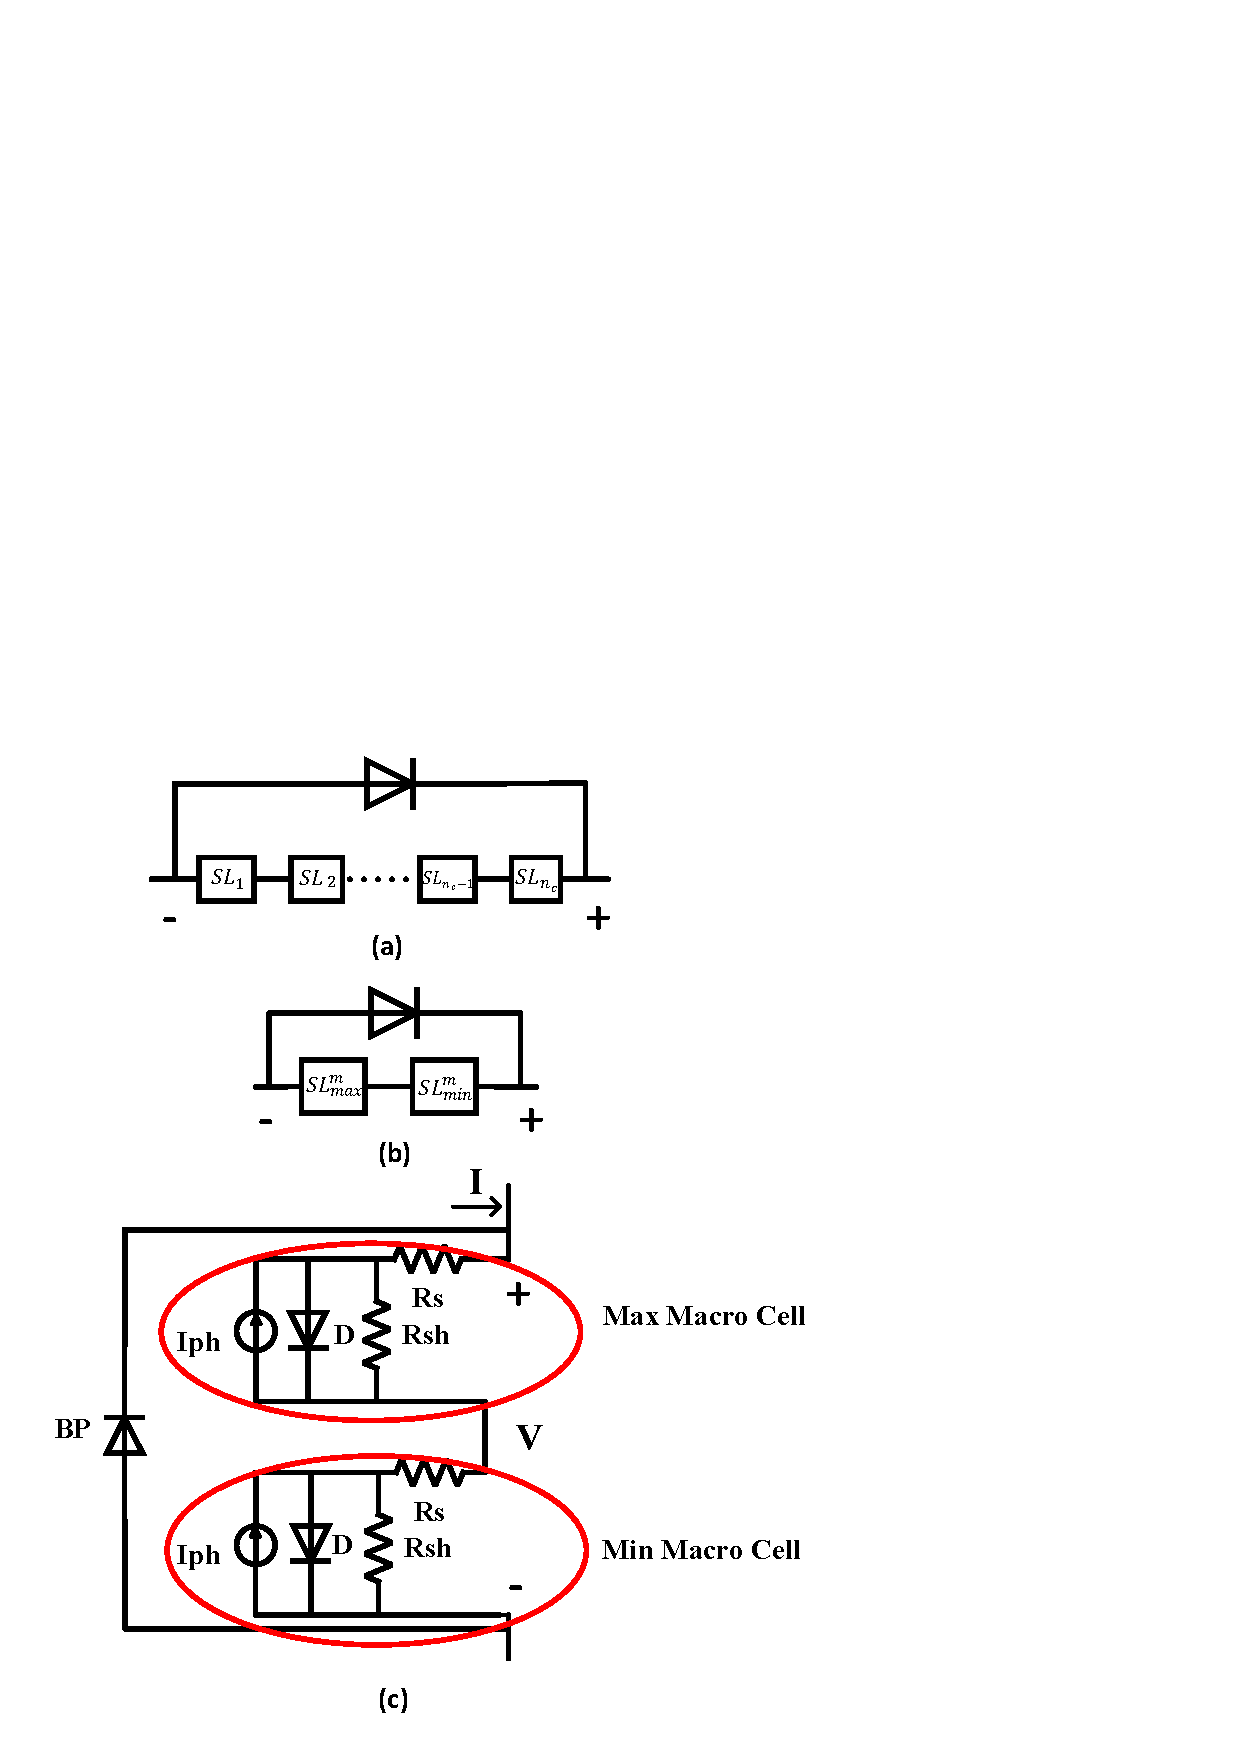
\includegraphics[width=1\columnwidth]{figs/cw_model_diagram.pdf}
    \caption{(a) One colony with $n_c$ solar cells (b) One colony model in Colony-Wise model (c) Circuit diagram of a colony modeled by Colony-Wise Model}
    \label{fig:cwDiagram}
\end{figure}

One colony in a PV module can always be represented as in Figure \ref{fig:cwDiagram} (a). Let us assume that this colony has $n_c$ solar cells. $SL_1$ to $SL_{n_c}$ denotes shading level of each solar cell. Recall that the Ground Truth model models each solar cell with a One-Diode model. Differ from the GT model, in the Colony-Wise model, all $n_c$ solar cells are lumped into at most two macro cells as shown in Figure \ref{fig:cwDiagram} (b). If $SL_1 = SL_2 = \dots = SL_{n_c}$, there is only one macro cell. Then all of the $n_c$ solar cells are lumped into this macro cell. Otherwise, all cells are lumped into two macro cells according to their shading levels (SLs). The two macro cells are also modeled by the One-Diode model, with their shading levels as $SL_{max}^m$ and $SL_{min}^m$. The superscript $m$ denotes the parameters are from macro cells. Section III B details the generation of parameters of the Colony-Wise model from the Ground Truth model. $SL_{max}^m$ and $SL_{min}^m$ are defined as the following:
\begin{equation}\label{equ:slMax}
  SL_{max}^m = \max_{i \in n_c}{SL_1, SL_2,  \dots, SL_{n_c} }
\end{equation}
\begin{equation}\label{equ:slMin}
  SL_{min}^m = \min_{i \in n_c}{SL_1, SL_2,  \dots, SL_{n_c} }
\end{equation}
\subsection{Parameter Generation of The Colony-Wise Model}
Heuristically, we pick up the two most representative solar cells within each colony to build the Colony-Wise model. These two cells are the basis of the two macro cells - the Max Macro Cell and the Min Macro Cell. These two macro cells are circled in the Figure \ref{fig:cwDiagram} (c). One cell ( to build the Max Macro Cell) has the maximum shading level $SL_{max}^m$, while the other cell (to build the Min Macro Cell) has the minimum shading level $SL_{min}^m$.

$n_{max}$ and $n_{min}$  counts the numbers of cells that belong to each macro cells within one colony. Note that:
\begin{equation}\label{equ:minMaxEqu}
  n_{max} + n_{min} = n_c
\end{equation}

The belonging of a cell depends on the shading level threshold:
\begin{equation}\label{equ:thres}
  thres = \frac{1}{2}(SL_{max}^m+ SL_{min}^m )
\end{equation}
For a solar cell, if its $SL \ge thres$, it belongs to the Max Macro Cell; otherwise, it belongs to the Min Macro Cell.

The circuit diagram of a colony modeled by the Colony-Wise model is as shown in Figure \ref{fig:cwDiagram} (c). We can derive the parameters of Max Macro Cell and Min Macro Cell based on $n_{max}$ and $n_{min}$. This model reduction is shown in Table \ref{table:cwRule}.

\begin{table}[tb]
  \caption{Model Reduction Rule for the Colony-Wise Model }
  \label{table:cwRule}
  \centering
  \normalsize
\begin{tabular}{|l|l|l|}
  \hline
  Parameter & Max Macro Cell & Min Macro Cell \\
  \hline
  $I_{ph}^m$ & $SL_{max}^m$ & $SL_{min}^m$ \\
  \hline
  $I_s^m$ & $I_{s_o}$ & $I_{s_o}$ \\
  \hline
  $N^m$ & $n_{max}*N_o$ & $n_{min}*N_o$ \\
  \hline
  $R_s^m$ & $n_{max}*R_{s_o}$ & $n_{min}*R_{s_o}$ \\
  \hline
  $R_{sh}^m$ & $R_{sh_o}$ & $R_{sh_o}$ \\
  \hline
\end{tabular}
\end{table}





\section{The N-Colony PV Module Model}
\subsection{The N-Colony Model Equivalent Circuit Diagram}
For a PV module with homogenous bypass diode distribution (each chain in a PV module has the same number of bypass diodes, and these bypass diodes have the same configuration), we can further lump its Ground Truth model into the N-Colony model. The notation $N$ stands for the number of bypass diodes in each chain. In this paper, we use notation from Section II C, $N = n_{bp}$.

\begin{figure}[tb]
    \centering
    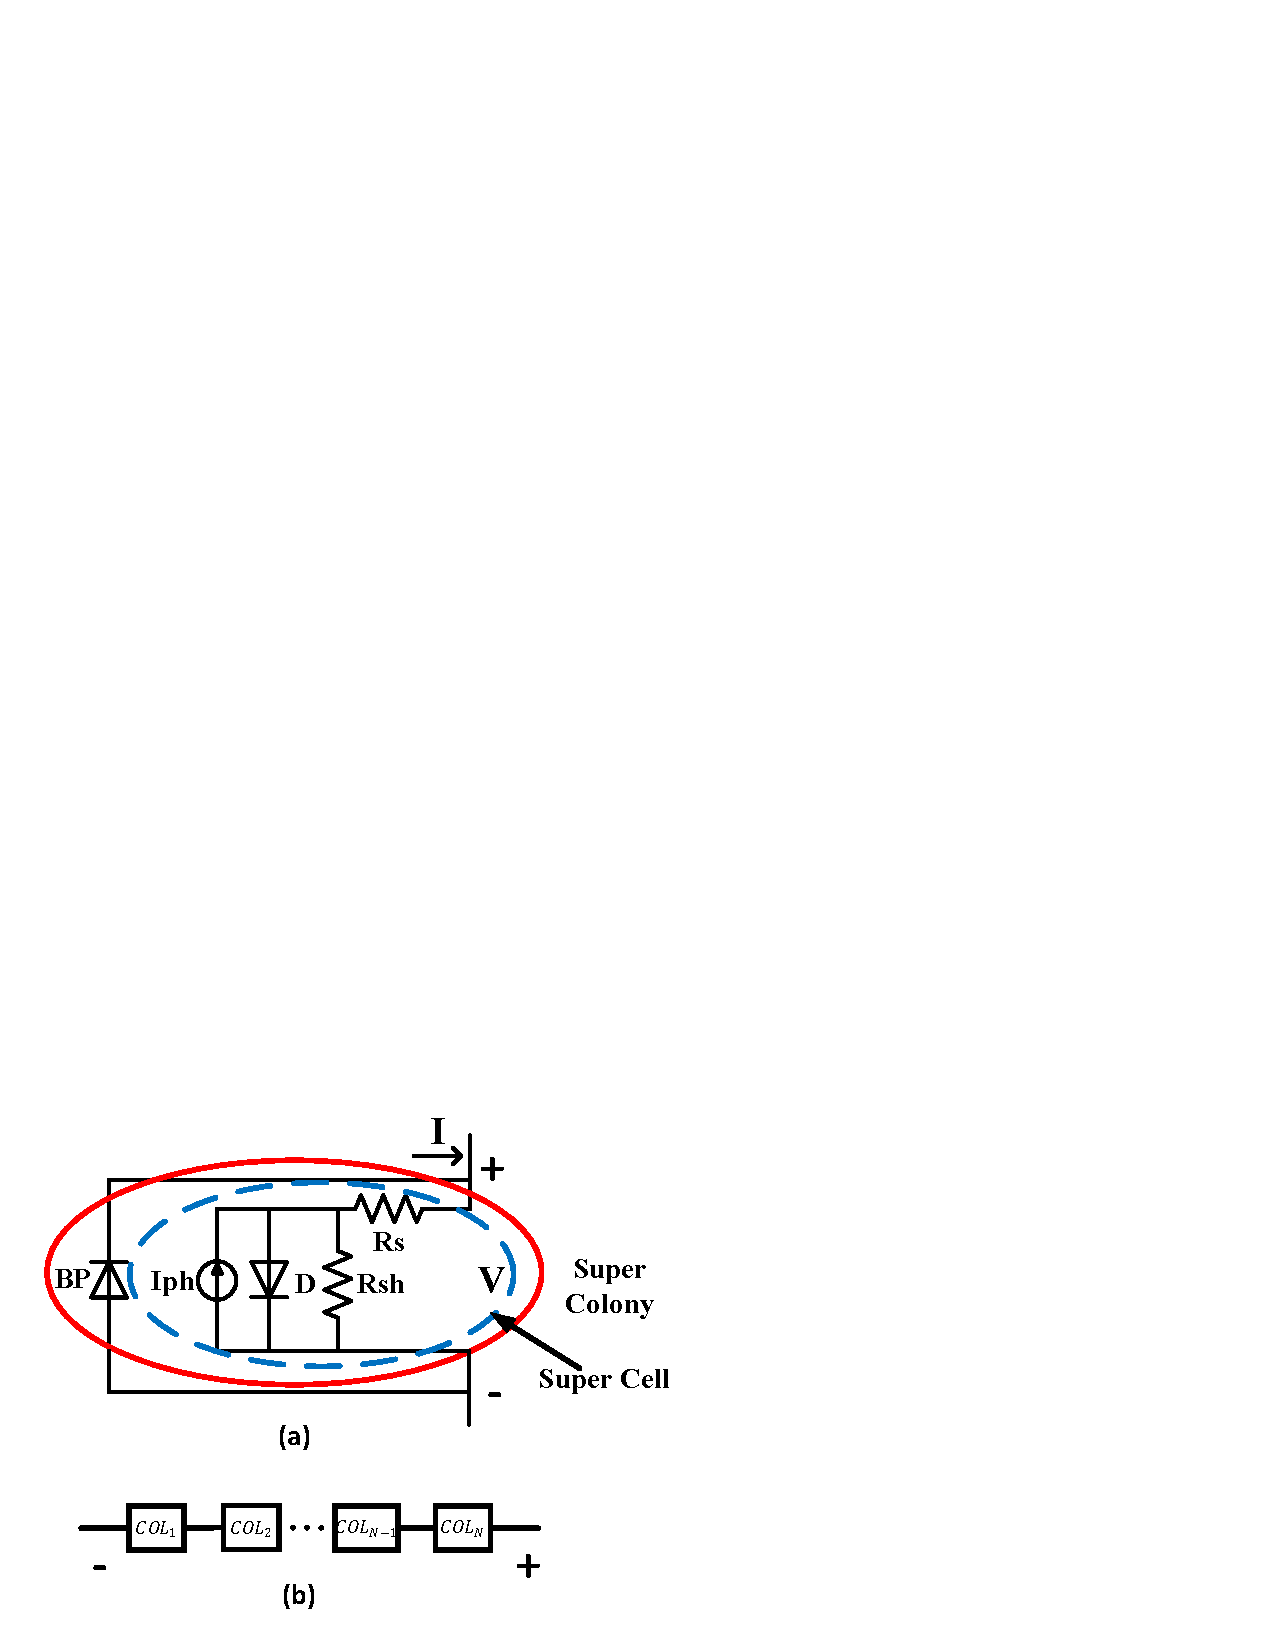
\includegraphics[width=1\columnwidth]{figs/nc_model_diagram.pdf}
    \caption{(a) Equivalent circuit of one super colony in the N-Colony model (b) Diagram of the N-Colony model of a PV module}
    \label{fig:ncDiagram}
\end{figure}

The N-Colony Model consists of $N$  \textit{super colonies}. Each super colony consists of one bypass diode and one \textit{super cell}. The super sell is as circled in Figure \ref{fig:ncDiagram}, and is again modeled by the One-Diode Model. The equivalent circuit diagram for one such colony is shown in Figure \ref{fig:ncDiagram} (a). The N-Colony model of a $mSnP$ PV module is as shown in Figure \ref{fig:ncDiagram} (b).

The N-Colony model is an heuristic model based on experiments. The parameters of the N-Colony modele need to be curve fitted from the Ground Truth model. The details of the parameter generation are shown in the next sub-section.
\subsection{Parameter Generation of the N-Colony Model}
\subsubsection{Super Colony's Shading Level Generation}
First, we determine the shading level of each super colony. It is also the $I_{ph}$ of the One-Diode model in the super cell.

According to Equation \ref{equ:slMax} and \ref{equ:slMin}, we can calculate the $SL_{max}^{(i,j)}$ and the $SL_{min}^{(i,j)}$ of each colony. Note that when the cells are identical within a colony, $SL_{max}^{(i,j)} = SL_{min}^{(i,j)}$ . The notation $(i,j)$ represents the $i^{th}$ colony in the $j^{th}$ column in a PV module.

We define a matrix namely the All-Min-Matrix ($M_{am}$) to record all $SL_{min}^{(i,j)}$s. $M_{am}$ has orders, and is formed as the following. For the $j^{th}$ chain of a PV module, we have the a SL sequence for all the colonies within this chain: $SL_{min}^{(1,j)},SL_{min}^{(2,j)}m \dots,SL_{min}^{(n_{bp},j)}$. We then reorder this sequence into: $SL^{(1,j)},SL^{(2,j)}, \dots,SL^{(n_{bp},j)}$, such that:
\begin{equation}\label{equ:slChain}
  SL^{(1,j)} \le SL^{(2,j)} \le \dots \le SL^{(n_{bp},j)}
\end{equation}
The All-Min-Matrix then is defined accordingly:
\begin{equation}\label{equ:Mam}
M_{am} =
\begin{bmatrix}
 SL^{(1,1)} & \dots & SL^{(1,n)} \\
 \dots & \dots & \dots \\
 SL^{(n_{bp},1)} & \dots & SL^{(n_{bp},n)} \\
\end{bmatrix}
\end{equation}
where $n$ is the number of solar cell chains in a $mSnP$ PV module.

Finally, for the $i^{th}$ super colony in the N-Colony model, its $I_{ph}^i$ is generated by Equation \ref{equ:scIph}:
\begin{equation}\label{equ:scIph}
  I_{ph}^i = \sum_{j=1}^n{M_{am}(i,j)}
\end{equation}

\subsubsection{Cell Shading Ratio, Colony Shading Ratio and Shading Ratio}
We define three variables that are the backbone parameters in the N-Colony model: the Shading Ratio ($R$), the Cell Shading Ratio ($c_r$) and the Colony Shading Ratio ($C_R$). Parameters in N-Colony are generated from $R$, and $R$ depends on $c_r$ and $C_R$. For a PV module that has $n_{bp}$ bypass diodes in a solar cell chain, we have $c_r^1, c_r^2, \dots, c_r^{n_{bp}}$, $C_R^1,C_R^2,\dots,C_R^{n_{bp}}$ and $R^1,R^2,\dots,R^{n_{bp}}$ for a PV module.

$c_r$ and $C_R$ are defined as in Equation \ref{equ:crCR}:
\begin{equation}\label{equ:crCR}
\begin{aligned}
  c_r^i & = \frac{\#i^{th}\ lv\ cell}{m*n} \\
  C_R^i & = \frac{\#i^{th}\ lv\ colony}{n*n_{bp}}
\end{aligned}
\end{equation}
where $\#i^{th}\ lv\ cell$ is the number of solar cells with shading level $i$. A solar cell has shading level $i$ when its SL satisfies:
\begin{equation}\label{equ:ithSLCell}
M_{am} (i-1, j) \le SL \le M_{am} (i, j)
\end{equation}
where $j$ is the column this solar cell belongs to.

Similarly, $\#i^{th}\ lv\ colony$ is the number of colonies with shading level $i$, which is defined as in Equation \ref{equ:ithSLCol} :
\begin{equation}\label{equ:ithSLCol}
M_{am} (i-1, j) \le SL_{min} \le M_{am} (i, j)
\end{equation}
where $j$ is the column this colony belongs to, and $SL_{min}$ is defined in Equation \ref{equ:slMin}.

$R$ is then defined as:
\begin{equation}\label{equ:rDef}
R^i =
    \begin{cases}
      \alpha_i*c_r^i+ \beta_i*C_R^i+ \gamma_i  & \text{if}\  i \neq n_{bp}\\
      1 - \sum_{j = 1}^{n_{bp}-1}{R^i} & \text{otherwise}
     \end{cases}
\end{equation}
where $\alpha_i$, $\beta_i$ and $\gamma_i$ are the weighing factors that need to be curve fitted. Note that we need to make sure all $R^i$s are greater then zero.

Therefore, for a PV module with $n*n_{bp}$ bypass diodes on each chain, $(n*n_{bp} - 1)*3$ parameters are required to be curve fitted.


\subsubsection{Parameters in the N-Colony Model}
Once we have all $R^i$s and $I_{ph}^i$s, we can generate all N-Colony model parameters based on Table \ref{table:ncRule}.
\begin{table}[tb]
  \caption{Model Reduction Rule for the N-Colony Model }
  \label{table:ncRule}
  \centering
  \normalsize
\begin{tabular}{|l|l|}
  \hline
  Parameter & Super Colony $i$ \\
  \hline
  $I_{ph}^s$ & $I_{ph}^i$ \\
  \hline
  $I_s^s$ & $I_{s_o}*n*R^i $\\
  \hline
  $N^s$ & $N_o*m*R^i $\\
  \hline
  $R_s^s$ & $R_{s_o}*m/n*R^i$ \\
  \hline
  $R_{sh}^s$ & $R_{sh_o}/n*R^i$  \\
  \hline
  $I_{s_{bp}}^s$ & $I_{s_{bp_o}}*n*R^i$  \\
  \hline
  $N_{bp}^s$ & $N_{bp_o}*n*R^i$  \\
  \hline
\end{tabular}
\end{table}
In Table \ref{table:ncRule}, $I_{s_{bp}}^s$ and $N_{bp}^s$ are parameters of the bypass diode in the super colony. The other parameters are for the super cell. The superscript $s$ denotes the corresponding parameters are from the super colony.

\begin{table*}[tb]
  \caption{Curve Fitting Results of the N-Colony Model}
  \label{table:ncCurveFit}
  \centering
  \normalsize
\begin{tabular}{|l|l|l|l|}
  \hline
  Weighting Factors & $60s2p$ & $30s4p$ & $40s2p$\\
  \hline
  $\{\alpha_1, \beta_1, \gamma_1\}$ &$\{0.41, 0.17, 0.04\} $ & $\{0.75, 0.22, 0.06\} $ & $\{0.71, 0.27, 0.10\}$ \\
  \hline
  $\{\alpha_2, \beta_2, \gamma_2\}$ &$\{0.40, 0.20, 0.14\} $ & $NA $ & $NA$ \\
  \hline
\end{tabular}
\end{table*}


\subsubsection{Curve Fitting of the Weighting Factors}
The goal of the N-Colony model is to minimize the error between its Power-Voltage (PV) curve and the curve generated by the Ground Truth model. In addition, we care about the maximum power point (MPP), which is the optimal operation point of a PV module. Therefore, the objective function of the curve fitting is described in Equation \ref{equ:cfObj}.
\begin{equation}\label{equ:cfObj}
Obj = w_1*0.5*(1-CORR)+ w_2*Error_{MPP}
\end{equation}
where $Error_{MPP}$ is the relative error of the maximum power point (MPP), and CORR is the correlation of the two curves. If we have two P-V curves, namely $X$ and $Y$, with each curve consisting of sampled points $x_i$ and $y_i$, $i=1,2,\dots,n$, then the CORR of the two curves is defined in Equation \ref{equ:corrDef}.
\begin{equation}\label{equ:corrDef}
CORR = \frac{\sum_{i=1}^n{(x_i - \bar{x})(y_i - \bar{y}) } } {\sqrt{\sum_{i=1}^n{(x_i - \bar{x})^2}}\sqrt{\sum_{i=1}^n{(y_i - \bar{y})^2}}}
\end{equation}
where $\bar{x}$ and $\bar{y}$ are the average value for all $x_i$ and $y_i$. Note that the closer $CORR$ is to $1$, the more similar the two curves are.

In addition, to quantify the impacts of these two optimization goals, they have to be normalized. $Error_{MPP}$ has already been normalized because its value is between $0$ and $1$. However, CORR has a range between $-1$ and $1$. Therefore, the $0.5*(1-CORR )$ term is the normalization term used in Equation \ref{equ:cfObj}. Furthermore, $w_1$  and $w_2$ are weights that are used to count for the impacts of CORR and MPP after normalization. In our experiment, they are both set to $0.5$ to make the impacts of CORR and MPP equal.

\subsection{Computational Complexity of the N-Colony Model}
The complexity between the GT model and the NC model can also be roughly estimated by Equation \ref{equ:diodeRatioGTNC}, following the same reasoning in Section III C. The NC model has constant computational complexity in the sense of $n_{bp}$. $n_{bp}$ is usually a fixed small number.
\begin{equation}\label{equ:diodeRatioGTNC}
  diode\_ratio = \frac{m*n+n*n_{bp}}{n_{bp}*2}
\end{equation}

%\subsection{Table-based N-Colony Model}
%The N-Colony model has high efficiency. Furthermore, if there are only $2$ bypass diodes in a solar cell chain, we can build a Table-based N-Colony model.
%
%Under the above assumption when $n_{bp}=2$, only four key variables: $c_r$, $C_R$, $I_{ph}^1$ and $I_{ph}^2$, are enough to derive all parameters in the N-Colony model. For a $mSnP$ PV module, the combination of $c_r$ equals $m*n$, $C_R$ equals $2^{2m}$ and both $I_{ph}^1$ and $I_{ph}^2$ equal $n_{sl}*m$, where $n_{sl}$ is the number of shading levels a PV model have. Therefore, this model can be pre-calculated and stored into a four-dimensional table. In addition, computing time for each variable-combination is constant, which makes the table build-up time to be scalable. For a given shading pattern, the P-V curve can be estimated by table lookup according to the four variables. Fetching data from table needs only a small and constant complexity, which is very efficient.













\section{Experimental Results}
\subsection{Experiment Settings}
In this section, we compare three models for PV modules in terms of accuracy and speed. These models are the Ground Truth (GT) model, the Colony-Wise (CW) model, and the N-Colony (TC) model. Without losing generality, we assume that all the cells that have the same shading level within one PV module are adjacent to each other.

We use notations from Section II (Equation \ref{equ:slRepresent}) to represent the multilevel shading settings. In the experiment, we assume $SLs = \{2A, 1.75A, 1.5A, 1.25A, 1A\}$. In order to simulate multiple shading scenarios, we define a ration array that consist three ratios:
$ratios1 = \{70\%, 10\%, 5\%, 5\%, 10\%\}$,
$ratios2 = \{50\%, 10\%, 10\%, 10\%, 20\%\}$ and
$ratios1 = \{20\%, 20\%, 20\%, 20\%, 20\%\}$. The three $ratios$ covers low shading, medium shading and high shading respectively. For one PV module with each shading ratio, we generate $100$ random shading patterns to evaluate three models.

We instantiate three different PV modules in our experiment: $60s2p$, $30s4p$ and $40s2p$. As for the bypass diode configuration, every $15$ to $20$ cells have one bypass diode according to \cite{bp1}. Therefore, $60s2p$ module has $3$ bypass diodes for each chain, and other two modules have $2$ bypass diodes for each chain. We use the same solar cell's One-Diode model parameters as in \cite{oneD1}. Diode quality factor $N_o=1.5$, diode saturation current $I_{s_o}=10^{-6}A$, serial resistance $R_{s_o}=0.0079\Omega$ and shunt resistance $R_{sh_o} = 5000\Omega$. The bypass diode has the quality factor $N_{bp_o} = 1$ and saturation current $I_{sbp_o}= 10^{-6}A$.

The circuit simulations are conducted in HSPICE \cite{hspice}. The experiment was conducted on a laptop that has an Intel $i5$ $2.4$GHz CPU, and $8$GB memory.

For the N-Colony model, $20$ shading patterns are used to curve fit the weighting factors in Equation \ref{equ:cfObj}. The resulting parameters are used to validate the PV module models through the rest of shading patterns. We implemented the gradient descent search to achieve the curve fitting. In order to jump out of the local optimal, several randomized initial points were used and we picked the best results. The curve-fitted parameters of the NC model are shown in Table \ref{table:ncCurveFit}. Although they are different for different PV modules, the curve fitting overhead is reasonable because in a solar farm, the types of PV modules are usually small.

Furthermore, $\alpha$ is always larger than $\beta$ and $\gamma$ under all conditions. This shows that $C_R$ has a larger impact on PV module modeling than $c_r$. $C_R$ is the dominant factor in a PV module��s output power. This implies that the PV module generates less power, when the shade covers more colonies while the area of the shade remains the same. Similar observations can also be found in other references \cite{villalva2009comprehensive, oneD1, oneD3}.


\subsection{Accuracy Comparisons Among the Three Models}



To evaluate accuracy of the Colony-Wise model and the N-Colony model, the average relative error of the Maximum Power Point (MPP) and the average P-V curve correlation (CORR) are compared with the Ground Truth model. The MPP represents the operation point of a PV module, and the CORR shows the similarity between the estimated P-V curve and the Ground Truth curve.

\begin{figure}[tb]
    \centering
    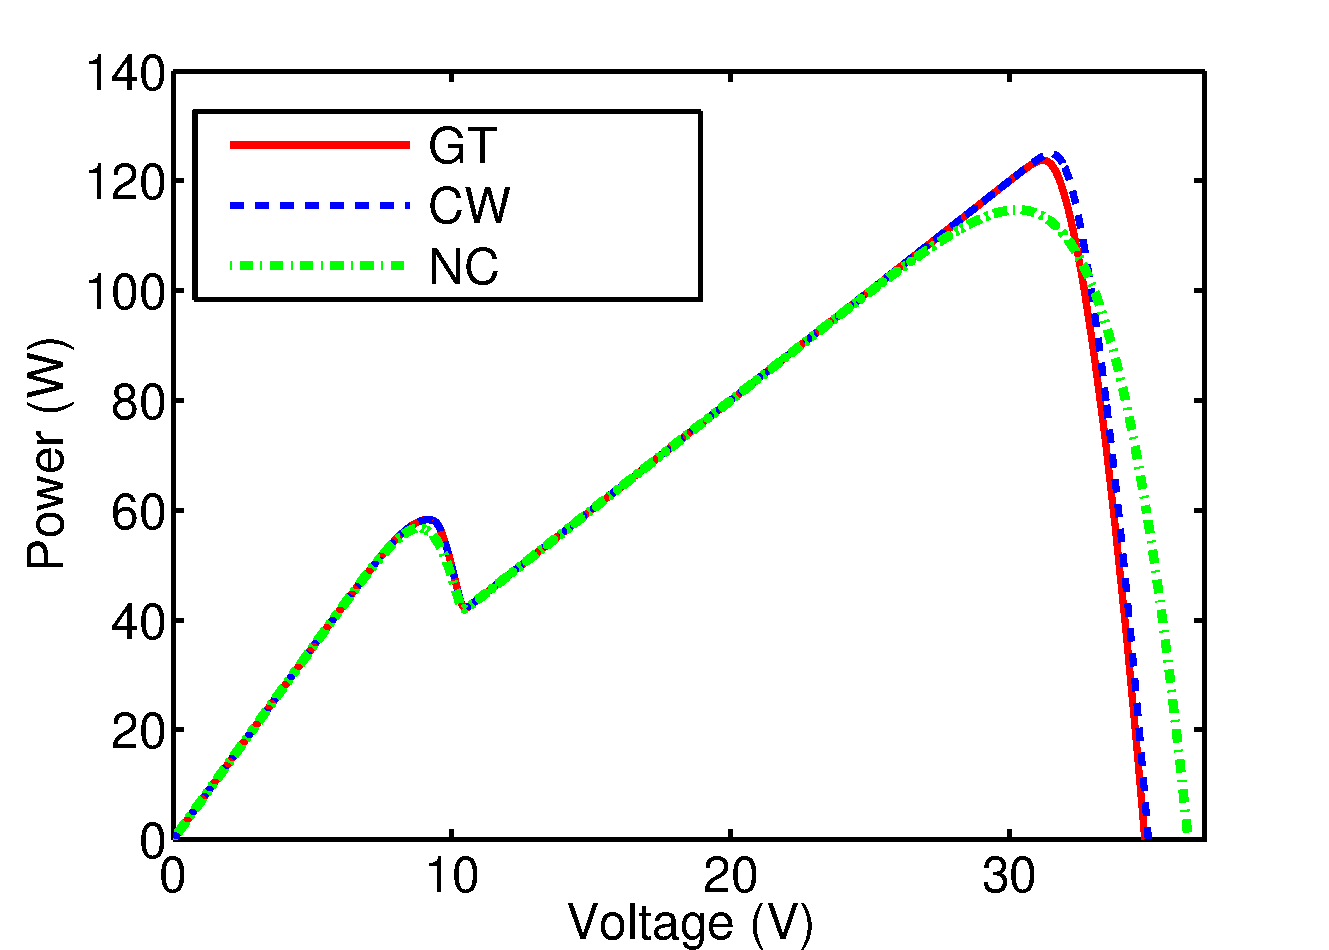
\includegraphics[width=0.8\columnwidth]{figs/pvExample.pdf}
    \caption{An example of three P-V curves generated by three models of a same PV module configuration}
    \label{fig:pvExample}
\end{figure}

\begin{figure}[tb]
    \centering
    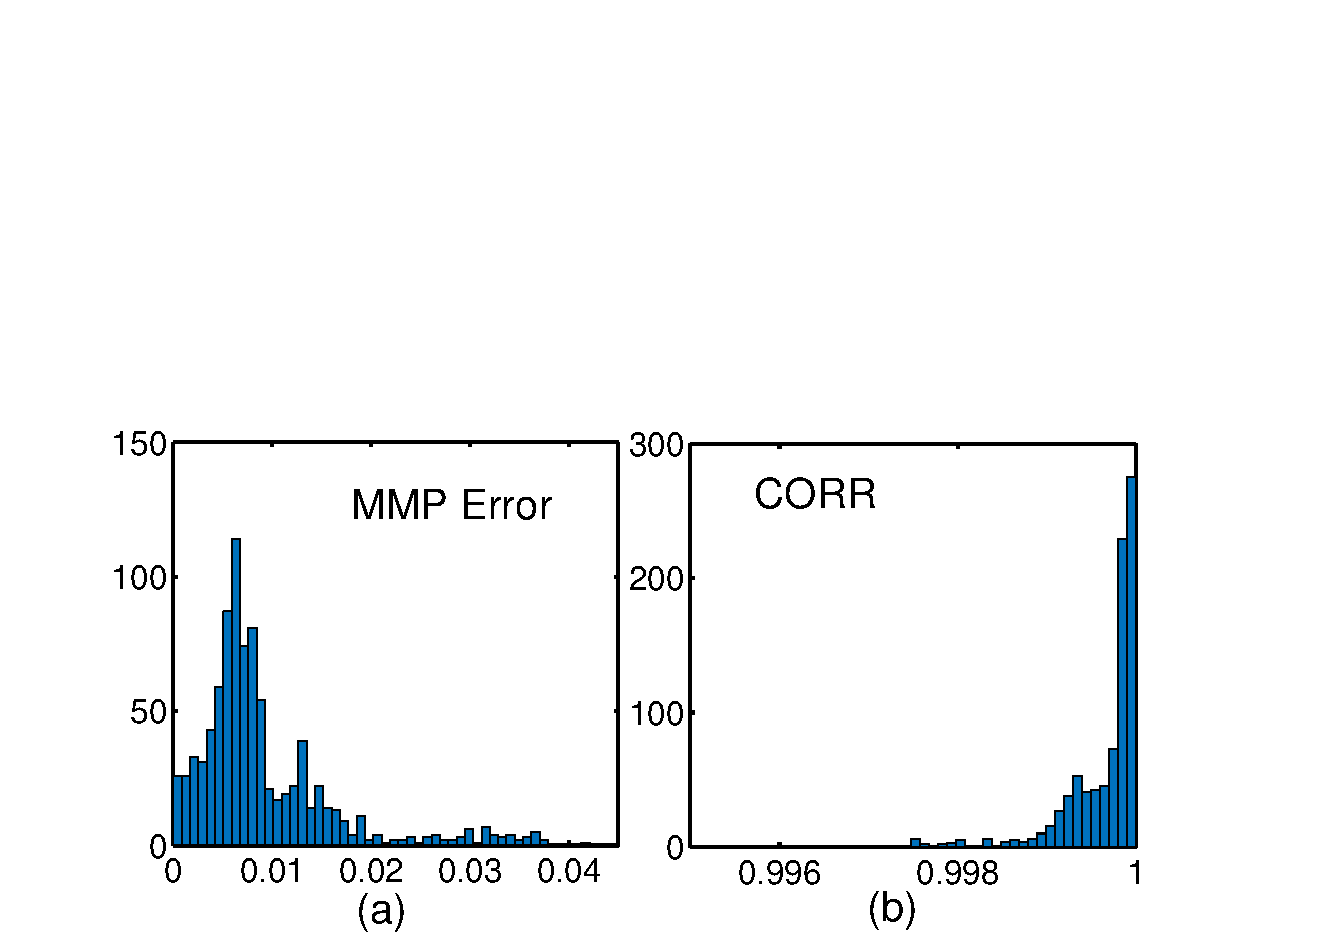
\includegraphics[width=1\columnwidth]{figs/cwHist_5lvl.pdf}
    \caption{(a) CW model's MPP error histogram over $900$ test cases (b) CW model's CORR histogram over $900$ test cases}
    \label{fig:cwHist}
\end{figure}

Figure \ref{fig:pvExample} shows an typical example of the P-V curves generated by the three models. The PV module is $60s2p$ with $3$ bypass diodes for each solar cell chain. Compared to the Ground Truth model's P-V curve (red solid line), the Colony-Wise model (blue dashed line) has almost the same accuracy, while the N-Colony model (green dot-dashed line) sacrifices the model a little bit to trade off for the constant computational speed.

First, we compare the Colony-Wise model with the Ground Truth model over the $900$ test cases. Figure \ref{fig:cwHist} (a) (b) show the histogram of $900$ cases�� MPP error and CORR. The average MPP error is $0.92\%$, and the average CORR is $0.999$. In addition, the largest MPP error is $4.21\%$, $95\%$ of MPP errors are less than $2.60\%$, and the lowest CORR
is $0.995$. The results show that the Colony-Wise model has nearly the same accuracy as the Ground Truth model.

\begin{figure}[tb]
    \centering
    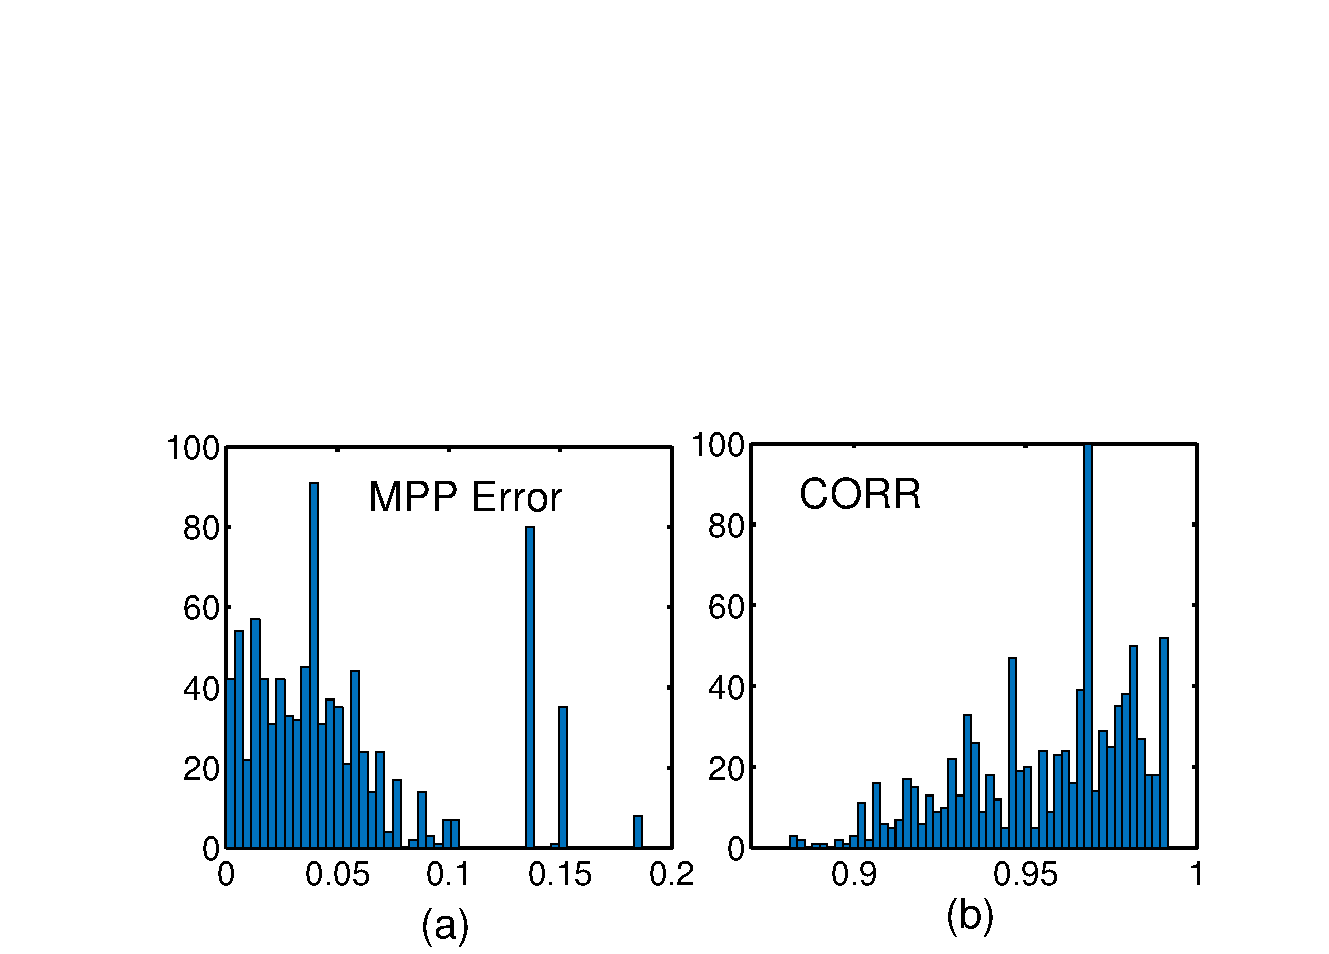
\includegraphics[width=1\columnwidth]{figs/ncHist_5lvl.pdf}
    \caption{(a) NC model's MPP error histogram over $900$ test cases (b) NC model's CORR histogram over $900$ test cases}
    \label{fig:ncHist}
\end{figure}

Then, we compare the N-Colony model with the Ground Truth model. Figure \ref{fig:ncHist} (a) shows the histogram of $900$ cases�� MPP error and (b) shows the CORRs' histogram. The average MPP error is $5.15\%$, and the average CORR is $0.96$. The NC model sacrifices the accuracy a little for it's constant computational complexity. There are two major reasons for the loss of accuracy. First, the NC model has constant number of component, therefore, there will be information loss when converting from the GT model to the NC model. Second, the NC model is an experimental model, which means some of its parameters are curved fitted (trained) through experiment data. The shading patterns of the large error cases are not covered in the $20$ training patterns. Therefore, the NC model has larger error for these cases. To overcome this weakness, we can increase the number of training patterns.

\begin{table}[tb]
  \caption{Runtime of the Three Models}
  \label{table:rtComp}
  \centering
  \normalsize
\begin{tabular}{|l|l|l|l|}
  \hline
  \pbox{2cm}{PV Module \\ Config} & GT & CW (Speedup) & NC (Speedup)\\
  \hline
  $60s2p$ &$2216s$ & $318s$ (7.0X) & $129s$ (17.2X)\\
  \hline
  $30s4p$ &$1325s$ & $317s$ (4.2X) & $91s$ (14.5X) \\
  \hline
  $40s2p$&$1652s$ & $267s$ (6.2X) & $101s$ (16.3X) \\
  \hline
\end{tabular}
\end{table}


\subsection{Speed Comparisons Among the Three Models}
We compare the three models' efficiency in terms of HSpice simulation time. The total run-time of the $300$ cases for each PV module is shown in Table \ref{table:rtComp}.

As shown in Table \ref{table:rtComp}, the runtime of the GT model is roughly proportional to the number of solar cells in a PV module. The runtime of the CW model is proportion to the multiplication of bypass diodes in a PV module. In addition, the runtime of the NC model is proportional to the number of bypass diodes in a solar cell chain.

The maximum speedup of the NC model is $17.2$X when the PV module setting is $60s2p$ ($3$ bypass diodes for each chain). The speedup can be higher when a PV module has more paralleled solar cell chain and less bypass diodes within one solar cell chain.















\section{Conclusions}
In this paper, two new PV module models are proposed, namely the Colony-Wise (CW) model and the N-Colony (NC) model. The two new models can support multiple shading levels on a PV module and various PV module configurations. The Colony-Wise model can efficiently capture the P-V curve of a PV module with almost no accuracy loss. The N-Colony model can further reduce the model��s computational complexity with a limited accuracy loss.

The N-Colony model is based on curve fitting. The accuracy of the model is highly related to the curve fitting process. Our future work will be finding optimal/good parameters in a high-dimensional solution space.






%
%{\small\textbf{Abstract---
% Abstract is a brief (50-80 word) synopsis of your paper.
%The purpose is to provide a quick outline of your
%presentation, giving the reader an overview of the
%research. It must be fit within the size allowed, which is
%about 3 inches or 7.5 centimeters.}}
%
%\section{Introduction}
%
%These introductions give you basic guidelines for preparing
%camera-ready papers for the ASP-DAC 2014. % Modified byK.S. Chong 25/08/13
%
%The instructions assume that you have computer that can generate an
%IEEE Xplore-compatible PDF file or any source file(s) which can be
%converted to PDF using IEEE PDF eXpress.
%
%These instructions have been prepared in the preferred format. For items
%not addressed here, please refer to recent issues of IEEE Transactions
%and simulate, as closely as possible.
%
%\section{How to Format the Page}
%
%\subsection{Paper Format}
%Prepare camera-ready paper in full size format, on 8.5'' $\times$ 11''
%(US Letter size) paper.
%
%\textbf{The width and height of the main text (including figures, tables, and
%footnotes, if any) is 181 mm (7.13 inches) and 250 mm (9.84 inches),
%respectively.}  Adjust the margins around the main text as follows;
%
%\begin{itemize}
%\item Top and bottom margins: 14.7 mm (0.58 inches).
%\item Left and right margins: 17.45 mm (0.685 inches).
%\end{itemize}
%
%There are two columns, 88 mm (3.465 inches) wide each, with 5 mm (0.2 inches)
%space between them (i.e., $88\mbox{ mm}\times2+5\mbox{ mm}=181\mbox{ mm}$).
%
%You should left- and right-justify your columns. On the last page of
%your paper, try to adjust the lengths of the two columns so that they
%are the same. Use automatic hyphenation if you have it and check
%spelling.
%
%%{\bf Number each of you submitted pages at the top, right corner, in
%%non-photographic light blue pencil.}
%
%\subsection{Fonts}
%The best results will be obtained if your computer word-processor has
%several font sizes. Try to follow the font sizes specified in Table I as
%best as you can. As an aid to gauging font size, 1 point is about
%0.35 mm. Use a proportional, serif font such as Times of Dutch Roman.
%
%\begin{table}[tb]
%\caption{Fonts for Camera-Ready Papers}
%\begin{minipage}{8cm}
%\def\arraystretch{1.5}\tabcolsep 2pt
%\def\thefootnote{a}\footnotesize
%\begin{tabular}{l@{~}l@{~~~}l}
%\hline
%\parbox[c]{7mm}{Font\newline Size} & Style & Text\\
%\hline
% 14pt&bold     &Paper title\\
% 12pt&         &Authors' names\\
% 10pt&         &Authors' affiliations, main text, equations,\\[-5pt]
%     &         &first letters in section titles\footnotemark[1]\\
% 10pt&italic   &Subheddings\\
% ~9pt&bold     &Abstract\\
% ~8pt&         &Section titles\footnotemark[1], table
%                names\footnotemark[1], first letters in table\\[-5pt]
%     &         &captions\footnotemark[1],
%                tables, figure captions, references,\\[-5pt]
%     &         &footnotes, text subscripts and superscripts\\
% ~6pt&         &Table captions\footnotemark[1], table superscripts\\
%\hline
%\end{tabular}
%\footnotetext[1]{\scriptsize Uppercase}
%\end{minipage}
%\end{table}
%
%\section{Figures and Tables}
%Position figures and tables at the tops and bottoms of columns. Avoid
%placing them in the middle of columns. Large figures and tables may
%span across both columns. Figure captions should be below the figures;
%table captions should be above the tables. Avoid placing figures and
%tables before their first mention in the text. Use the abbreviation
%``Fig.1'', even at the beginning of a sentence.
%
%\begin{figure}[tb]
%\begin{center}
%\begin{minipage}{5cm}
%$.$\hrulefill $.$\\$|$\hfill $|$\\$|$\hfill $|$\\$|$\hfill $|$\\
%$|$\hfill this is \hfill $|$\\
%$|$\hfill a sample \hfill $|$\\
%$|$\hfill  figure  \hfill $|$\\
%$|$\hfill $|$\\$|$\hfill $|$\\$|$\hfill $|$\\$.$\hrulefill $.$\\
%\end{minipage}
%\caption{This is a sample figure. Captions exceeding
%one line are arranged like this.}
%\end{center}
%\end{figure}
%
%\textbf{
%To meet the requirements for IEEE Xplore, the paper's graphics
%should have resolutions of 600dpi for monochrome, 300 dpi for
%grayscale, and 300 dpi for color.}
%
%\section{Helpful Hints}
%
%\subsection{References}
%List and number all references at the end of the paper. When referring
%to them in the text, type the corresponding reference number in the
%parentheses as shown at the end of this sentence \cite{key}. Number
%the citations consecutively. The sentence punctuation follows the
%parentheses. Do not use ``Ref.\cite{baz}'' or
%``reference\cite{baz}'' except at the beginning of a sentence.
%
%\subsection{Footnotes}
%Number the footnotes separately in superscripts. Place the actual
%footnote at the bottom of the column in which it is cited. Do not put
%footnotes in the reference list.
%
%\subsection{Authors names}
%
%Give all authors' names; do not use ``et al'' unless there are six
%authors or more. Papers that have not been published, even if they have
%been submitted for publication, should be cited as
%``unpublished''\cite{unpub}.  Papers that have been accepted for
%publication should be cited as ``in press''\cite{inpress}.
%Capitalize only the first word in a paper title, except for proper nouns
%and element symbols.
%
%For papers published in translation journals, please give the English
%citation first, followed by the original foreign language
%citations\cite{trans}.
%
%\subsection{Notice for \LaTeX\ users}
%
%If you use \LaTeX\ to create your camera-ready paper, we recommend you
%to use IEEE PDF eXpress (or \texttt{dvipdfm}) to produce PDF files from dvi
%files. If you cannot use it, please use Type1 fonts instead of ugly Type3 fonts!
%
%\section{Summary and Conclusions}
%
%This template can be downloaded through the ASP-DAC 2014 web site
%(http://www.aspdac.com/). If you have any problem, please contact ASP-DAC
%2014 publication chair\\
%(aspdac2014-pub@mls.aspdac.com). % Modified byK.S. Chong 25/08/13
%
%%this is how to do an unnumbered subsection
%\section*{\sc Acknowledgments}
%This article was written by referring to {\em ``Author's guide --
%Preparation of Papers in Two-Column Format for VLSI Symposia on
%Technology and Circuits''}, the {\em ``Preparation of Papers in
%Two-Column Format for the Proceedings of the 32nd ACM/IEEE Design
%Automation Conference''} written by Ann Burgmeyer, IEEE and {\em ``the
%template for producing IEEE-format articles using \LaTeX''}, written by
%Matthew Ward, Worcester Polytechnic Institute.
%
%\begin{thebibliography}{9}
%\footnotesize
%\bibitem{key}
%I. M. Author,
%``Some related article I wrote,''
%{\em Some Fine Journal}, vol. 17, pp. 1--100, 1987.
%
%\bibitem{baz}
%A. N. Expert,
%{\em A Book He Wrote,}
%His Publisher, 1989.
%
%\bibitem{unpub}
%M. Smith,
%``Title of paper optional here,''
%unpublished.
%
%\bibitem{inpress}
%K. Rose,
%``Title of paper with only first word capitalized,''	% bug fixed by M. Imai
%in press.
%
%\bibitem{trans}
%T. Murayama,
%``Title of paper published in translation journals,''	% bug fixed by M. Imai
%{\em Some English Journal}, vol. 17, pp. 1--100, 1995.	% bug fixed by M. Imai
%({\em Original Foreign Journal, vol. 1, pp. 100-200, 1993}.)	% ditto
%
%\end{thebibliography}



\begin{scriptsize}
    \bibliography{reference}
    \bibliographystyle{IEEEtran}
\end{scriptsize}

\end{document}

